%%%%%%%%%%%%%%%%%%%%%%%%%%%%%%%%%%%%%%%%%%%%%%%%%%%%%%%%%%%%%%%%%%%%%%%%%%%%%%%%
% IEEE Journal Paper
%%%%%%%%%%%%%%%%%%%%%%%%%%%%%%%%%%%%%%%%%%%%%%%%%%%%%%%%%%%%%%%%%%%%%%%%%%%%%%%%

\documentclass[journal]{IEEEtran}

\usepackage{amsmath,amssymb,amsfonts}
\usepackage{graphicx}
\usepackage{subcaption}
\usepackage{booktabs}
\usepackage{tabularx}
\usepackage{array}
\usepackage{multirow}
\usepackage{algorithm}
\usepackage{algpseudocode}
\usepackage{cite}
\usepackage{xcolor}
\usepackage{array}
\usepackage{float}
\usepackage{graphicx}
\usepackage{csvsimple}
\usepackage{array}
\usepackage{adjustbox}
\usepackage[compatibility=false]{caption}


\begin{document}

%%%%%%%%%%%%%%%%%%%%%%%%%%%%%%%%%%%%%%%%%%%%%%%%%%%%%%%%%%%%%%%%%%%%%%%%%%%%%%%%
\title{A Fuzzy-Supervised Hierarchical Soft Actor-Critic Energy Management Strategy for Floating Photovoltaic Hybrid Microgrids}

%%%%%%%%%%%%%%%%%%%%%%%%%%%%%%%%%%%%%%%%%%%%%%%%%%%%%%%%%%%%%%%%%%%%%%%%%%%%%%%%
%%%%%%%%%%%%%%%%%%%%%%%%%%%%%%%%%%%%%%%%%%%%%%%%%%%%%%%%%%%%%%%%%%%%%%%%%%%%%%%%

\author{%
Monowar~Mahmud$^{1}$,
Syed~Mohammad~Shamsul~Islam$^{2}$,
Author~3,
Author~4,
Author~5,
Mohammad~Nur-E-Alam$^{3,4}$%
%
\thanks{Monowar Mahmud is with the Department of Electrical and Electronic Engineering, Universiti Tenaga Nasional (UNITEN, The National Energy University), Kajang 43000, Selangor, Malaysia.}
%
\thanks{Syed Mohammad Shamsul Islam is with the School of Science, Edith Cowan University, 270 Joondalup Drive, Joondalup, WA 6027, Australia.}
%
\thanks{Author 3 is with [Affiliation].}
%
\thanks{Author 4 is with [Affiliation].}
%
\thanks{Author 5 is with [Affiliation].}
%
\thanks{Mohammad Nur-E-Alam is with the Space Science Centre, Institute of Climate Change, Universiti Kebangsaan Malaysia (UKM), 43600 Bangi, Selangor, Malaysia, and also with the School of Science, Edith Cowan University, 270 Joondalup Drive, Joondalup, WA 6027, Australia.}
%
\thanks{Corresponding author: XXXXX (e-mail: author@domain.edu).} % Optional
}
%%%%%%%%%%%%%%%%%%%%%%%%%%%%%%%%%%%%%%%%%%%%%%%%%%%%%%%%%%%%%%%%%%%%%%%%%%%%%%%%

\maketitle

\begin{abstract}
Floating photovoltaic (FPV) hybrid microgrids provide an affordable way of supplying electricity to remote riverine or marine locations; however, such microgrids need an adaptive energy management system to handle renewable intermittency, and supply reliability. In this paper, we present a novel method employing a hierarchical fuzzy supervised controller architecture where a safety constrained layer is integrated into the soft actor-critic deep reinforcement learning (DRL) methodology. In terms of performance, the proposed controller was able to attain 90.85\% FPV harvesting efficiency, the lowest operational cost (0.223~\$/kWh), and the lowest battery energy exchange (63.29~MWh) as compared to all benchmarking controllers while keeping the final state-of-health of the battery at 0.9848 without any violation of the State of Charge, battery power, and diesel power constraints. However, the reliability obtained (LPSP = 3.34\%) was inferior to the best optimization technique, pointing out the need for future work in reliability aware RL.
\end{abstract}

\begin{IEEEkeywords}
Floating photovoltaic (FPV), deep reinforcement learning (DRL), soft actor--critic (SAC), fuzzy logic.
\end{IEEEkeywords}

%%%%%%%%%%%%%%%%%%%%%%%%%%%%%%%%%%%%%%%%%%%%%%%%%%%%%%%%%%%%%%%%%%%%%%%%%%%%%%%%
\section{Introduction}

Floating photovoltaic (FPV) systems have emerged as an attractive renewable
energy technology for standalone and remote power systems because they utilize
otherwise unused water surfaces while improving photovoltaic (PV) efficiency through
the natural cooling effect of water \cite{Garrod2024,Temiz2022,Esparza2024}. When integrated with battery energy
storage systems (BESSs) and diesel generators (DGs), FPV-based hybrid
microgrids provide a practical and reliable solution for electrifying isolated
riverine and island communities where conventional grid expansion is
economically challenging \cite{Temiz2022,Gizaw2024}. However, the intermittent nature of PV sources, along with load uncertainty, demands the EMS must manage renewable power integration, battery operations, diesel power generation, cost of operations, and reliability in an ever-changing environment \cite{Garrod2024,Temiz2022,Esparza2024,Gizaw2024}.

Rule-based and fuzzy logic techniques, model predictive control (MPC) and online optimization methods are some of the commonly employed energy management system (EMS)s for managing power balance in these microgrids. Rule-based techniques are computation-efficient but cannot adapt properly to changing operating conditions, whereas fuzzy logic control is more robust using expert knowledge but depends on manual rule generation and exhibit poor learning performance in the long term \cite{Kumar2023,Kaysal2022}. On the other hand, MPC takes future operating conditions and system constraints into account. Thus, the computational cost becomes considerably high with respect to the prediction time frame and model accuracy \cite{Batiyah2020,Nair2020}. Similarly, the optimization-based methods, such as Grey Wolf Optimization and hybrid meta-heuristic algorithms, exhibit outstanding techno-economic results because of the solution to multi-objective optimization problems. Nonetheless, these optimization methods tend to have a significant number of computations to perform under varying conditions; hence, they are very costly from the computational perspective for FPV based microgrids \cite{Tukkee2024,Pramila2024}.

Recently, deep reinforcement learning (DRL) has attracted considerable attention for energy management because it enables adaptive online decision making without requiring an explicit system model. The DRL-based EMS developed recently has been able to achieve superior performance in terms of operational cost, renewable energy utilization, and battery management \cite{Ji2019,Guo2021,Meng2025}. However, standard DRL algorithms do not incorporate technical operating constraints but instead focus on optimizing long-term reward, thus making safe exploration and implementation difficult for isolated microgrids. Additionally, the trained policies are often non-interpretable and can fail in cases where unseen operating scenarios occur \cite{Garcia2015,Meng2025}. Hybrid controllers that integrate neural networks, fuzzy logic, or adaptive control techniques have enhanced transient stability and reliability. Yet, such systems have focused separately on each of these three factors, rather than incorporating all of them into a single online energy management scheme \cite{Aghmadi2025,Rajput2025,Adiche2024,Annamraju2021}.

To address these limitations, this study presents a new fuzzy-supervised hierarchical soft actor critic (SAC) EMS scheme specifically designed for the stand-alone FPV-based hybrid microgrid configuration. The scheme combines adaptive control learning, fuzzy supervisory reasoning, and safe action projection to maintain physically feasible battery and diesel operations while retaining the flexibility of DRL. The proposed controller is extensively simulated and found to extract high FPV utilization, minimum operational cost, minimum battery aging, and safe operation of the system.

The main contributions of this work are summarized as follows:

\begin{itemize}
\item Development of a hierarchical SAC-based EMS that integrates online DRL with fuzzy supervisory reasoning for standalone FPV hybrid microgrids.

\item Design of a safety-projection mechanism that guarantees physically feasible battery and diesel commands while satisfying operational constraints.
\end{itemize}


%%%%%%%%%%%%%%%%%%%%%%%%%%%%%%%%%%%%%%%%%%%%%%%%%%%%%%%%%%%%%%%%%%%%%%%%%%%%%%%%
\section{FPV Hybrid Microgrid Description}
%%%%%%%%%%%%%%%%%%%%%%%%%%%%%%%%%%%%%%%%%%%%%%%%%%%%%%%%%%%%%%%%%%%%%%%%%%%%%%%%

The investigated microgrid comprises a FPV, battery, and a diesel generator (DG). Figure \ref{fig:system_architecture} depicts the overall architecture with the centralized EMS. Wave- and wind-induced platform motion increases PV generation variations, making renewable power production more unreliable and real-time energy management more difficult in such cases. The battery is connected to the DC bus via a bidirectional DC-DC converter. The DG is connected directly to the AC bus of the microgrid. 
%%%%%%%%%%%%%%%%%%%%%%%%%%%%%%%%%%%%%%%%%%%%%%%%%%%%%%%%%%%%%%
\begin{figure}[!htbp]
    \centering
    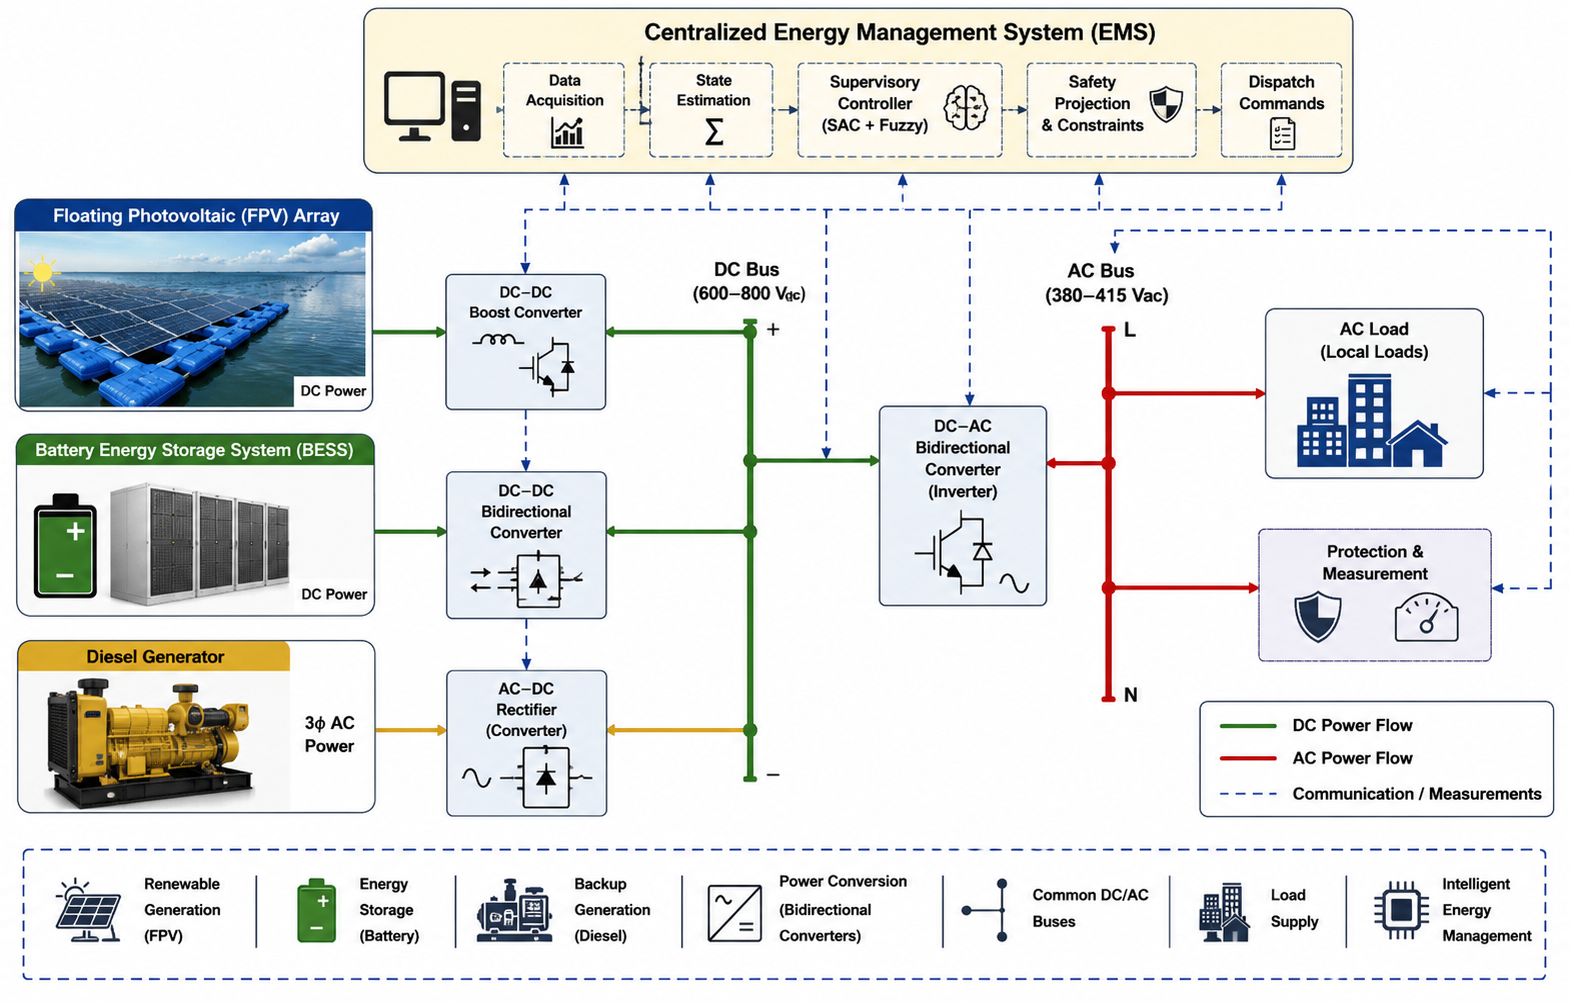
\includegraphics[width=\columnwidth]{Fig_1.png}
    \caption{Overall architecture of the FPV--battery--diesel hybrid microgrid and centralized energy management system (EMS).}
    \label{fig:system_architecture}
\end{figure}

The proposed controller is validated with the help of publicly accessible Central Hall microgrid data from the University of California San Diego (UCSD). This dataset contains multi-year synchronized data of electric load demand and photovoltaic generation sampled at an interval of 15 minutes \cite{silwal2021opensource}. Load and PV data is scaled based on the rated capacity of the considered FPV hybrid microgrid. As the original dataset corresponds to the standard rooftop PV system, the real-world conditions of FPV are mimicked with the addition of fluctuations in power due to pitch and roll of the platform. In addition, one-step ahead prediction of load and PV data is provided to the controller.

%%%%%%%%%%%%%%%%%%%%%%%%%%%%%%%%%%%%%%%%%%%%%%%%%%%%%%%%%%%%%%
\begin{table}[!ht]
\centering
\caption{Summary of the Central Hall dataset and simulation configuration.}
\label{tab:dataset}
\renewcommand{\arraystretch}{1.15}

\begin{tabularx}{\columnwidth}{>{\bfseries}l X}
\toprule
\multicolumn{2}{c}{\textbf{Dataset}}\\
\midrule
Source & UCSD Central Hall Microgrid \\
Reference & \cite{silwal2021opensource} \\
Sampling interval & 15 min \\
Duration & Multi-year \\
Measurements & Load demand, photovoltaic generation \\
Forecast & One-step ahead \\
\midrule
\multicolumn{2}{c}{\textbf{Simulation Configuration}}\\
\midrule
Microgrid & Floating photovoltaic (FPV)--Battery--Diesel hybrid microgrid \\
PV operating condition & Pitch- and roll-compensated photovoltaic generation \\
Simulation environment & Python (PyTorch) \\
Control interval & 15 min \\
Decision variables & Battery dispatch, diesel generation, photovoltaic curtailment, battery SOC target, and diesel commitment \\
\bottomrule
\end{tabularx}
\end{table}

%%%%%%%%%%%%%%%%%%%%%%%%%%%%%%%%%%%%%%%%%%%%%%%%%%%%%%%%%%%%%%%%%%%%%%%%%%%%%%%%
\section{Proposed Fuzzy-Supervised Hierarchical Soft Actor-Critic Energy Management Strategy}
%%%%%%%%%%%%%%%%%%%%%%%%%%%%%%%%%%%%%%%%%%%%%%%%%%%%%%%%%%%%%%%%%%%%%%%%%%%%%%%%
The proposed energy management strategy integrates SAC, fuzzy supervisory reasoning, and adaptive safety projections within a hierarchical decision-making architecture for FPV hybrid microgrids. The controller constantly updates the learned control law with expert supervisory knowledge prior to imposing adaptive constraints. Thus, the controller maintains the exploration ability of SAC and simultaneously enhances the utilization of renewable energy sources, battery lifespan, and economic efficiency. The overall architecture of the proposed controller is illustrated in Fig.~\ref{fig:controller}. For every control period, the controller evaluates the operation of the FPV hybrid microgrid and frames the energy management problem as a continuous-state continuous-action Markov Decision Process (MDP),

\begin{equation}
\mathcal{M}=(\mathcal{S},\mathcal{A},\mathcal{P},\mathcal{R},\gamma),
\label{eq:mdp}
\end{equation}

where $\mathcal{S}$, $\mathcal{A}$, $\mathcal{P}$, $\mathcal{R}$, and $\gamma$ represent the state space, action space, transition dynamics, reward function, and discount factor, respectively. The state space comprises the electrical load, PV generation, state of charge (SOC) of the battery, state of health (SOH) of the battery, previous action values, and forecasts of one-period ahead of load demand and PV generation. The output from the actor network is a continuous action vector that corresponds to battery dispatch, diesel generation, PV curtailment, battery SOC target, and diesel commitment.

\begin{figure*}[!ht]
\centering

%---------------- Row 1 ----------------%
\begin{subfigure}[t]{0.49\textwidth}
    \centering
    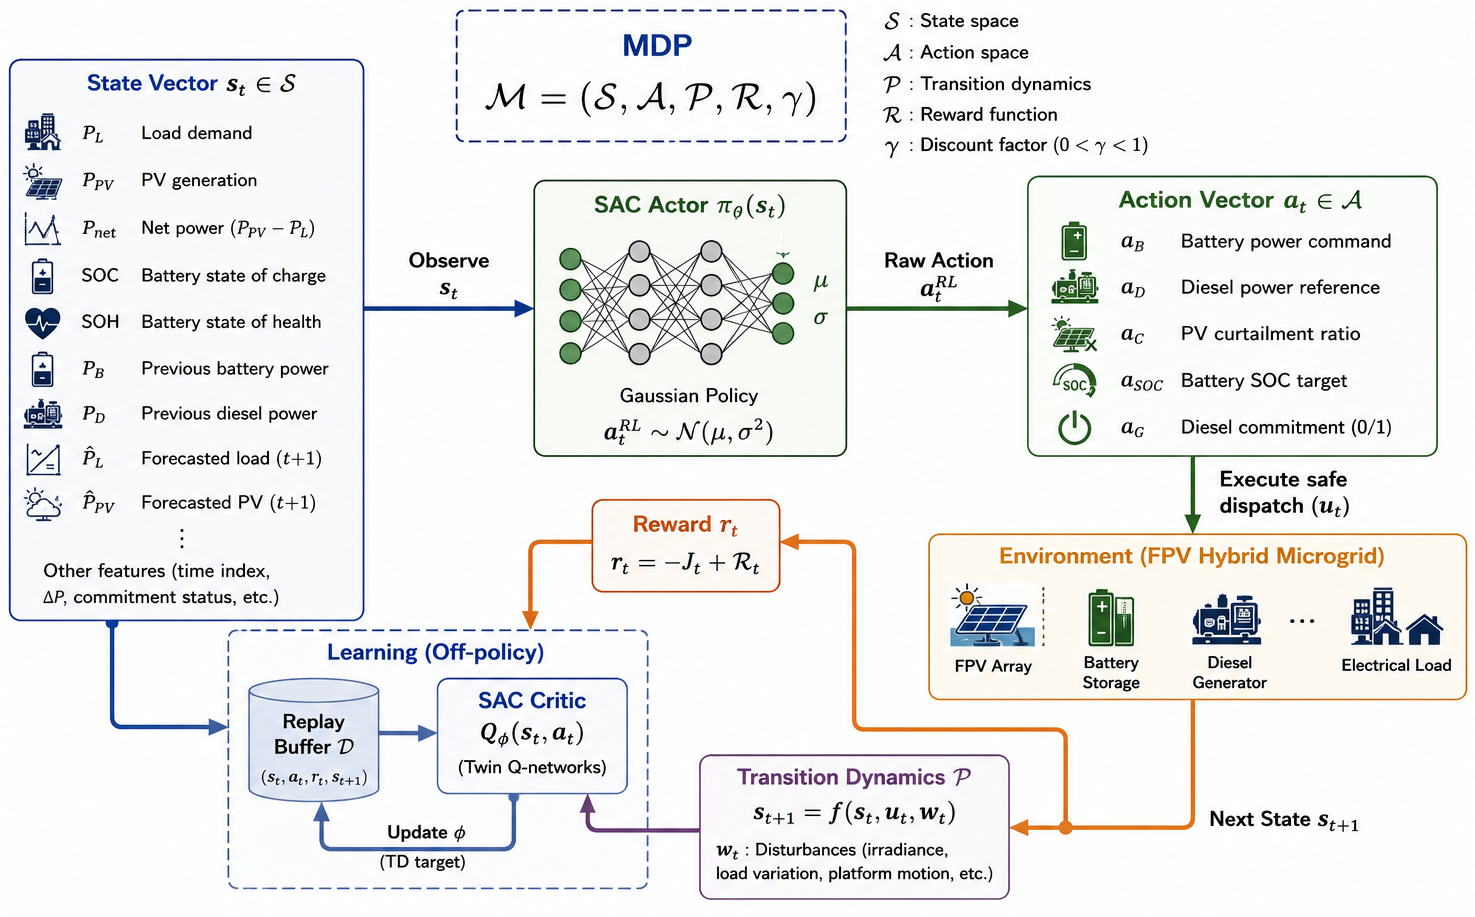
\includegraphics[width=\linewidth]{Fig_2a.png}
    \caption{Markov Decision Process formulation.}
    \label{fig:2a}
\end{subfigure}
\hfill
\begin{subfigure}[t]{0.49\textwidth}
    \centering
    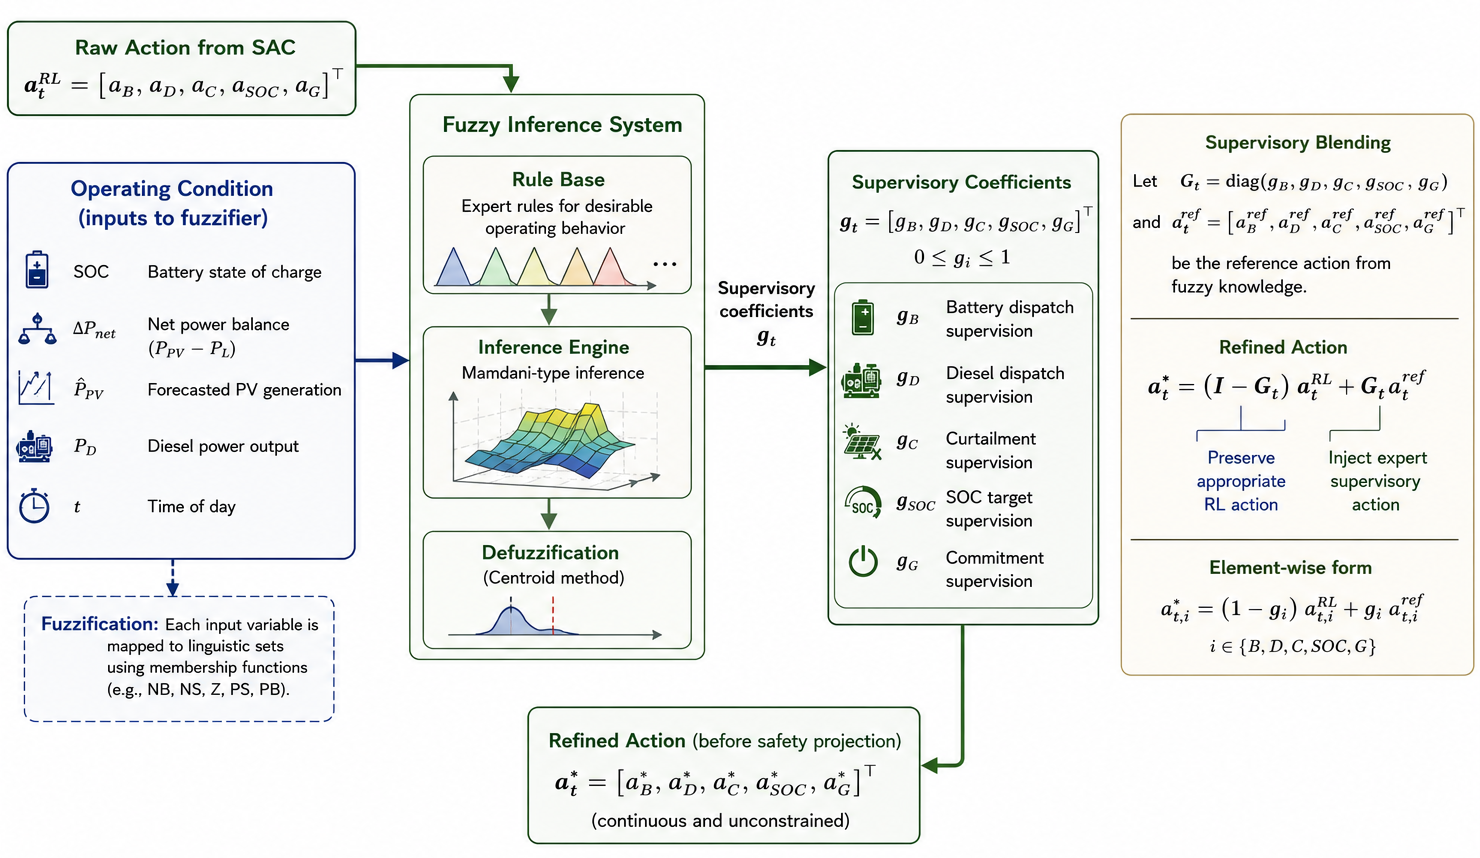
\includegraphics[width=\linewidth]{Fig_2b.png}
    \caption{Supervisory policy refinement.}
    \label{fig:2b}
\end{subfigure}

\vspace{2mm}

%---------------- Row 2 ----------------%
\begin{subfigure}[t]{0.49\textwidth}
    \centering
    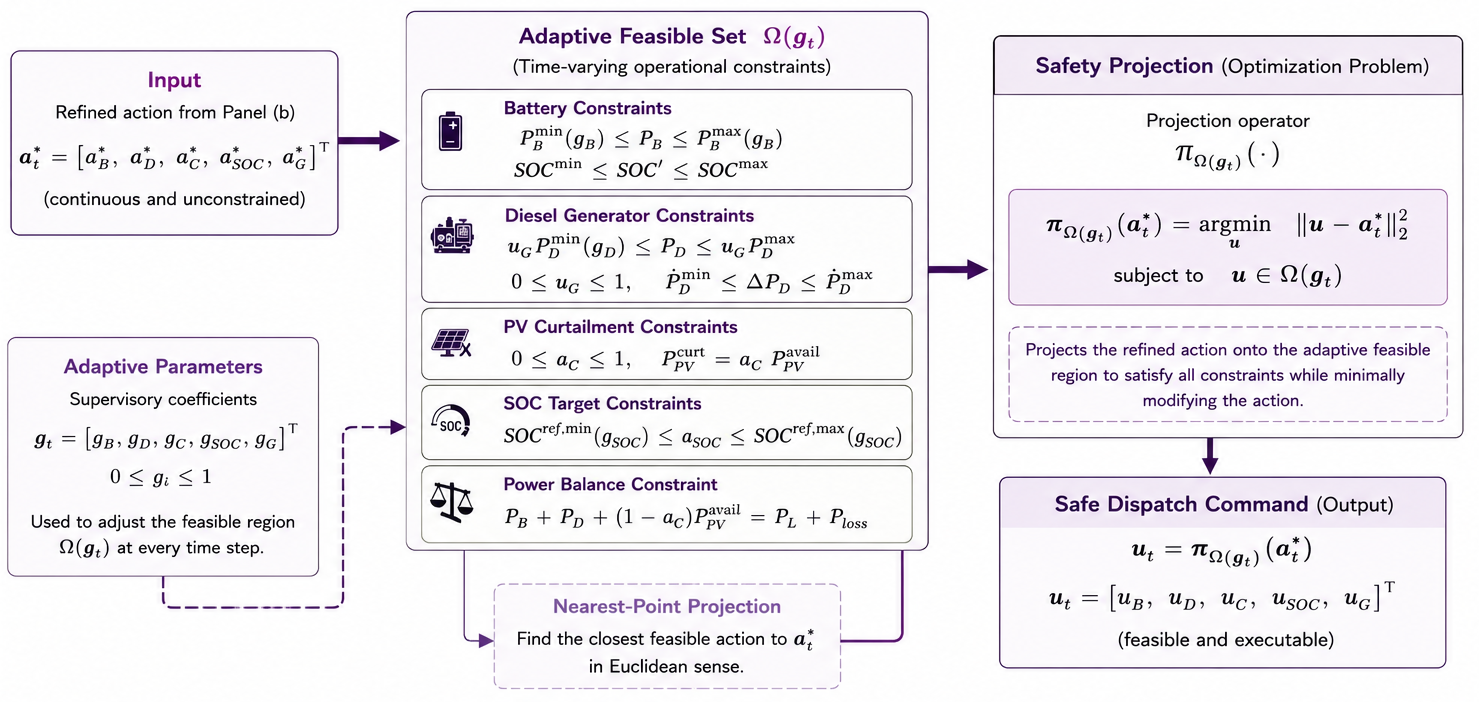
\includegraphics[width=\linewidth]{Fig_2c.png}
    \caption{Adaptive safety projection.}
    \label{fig:2c}
\end{subfigure}
\hfill
\begin{subfigure}[t]{0.49\textwidth}
    \centering
    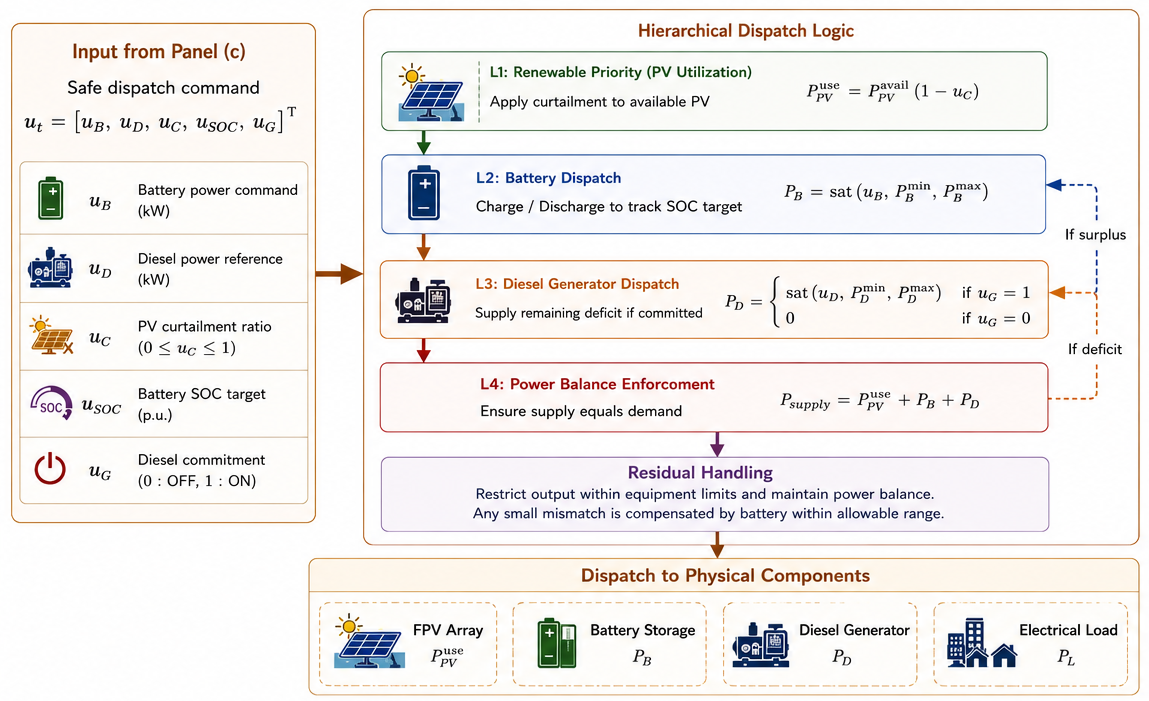
\includegraphics[width=\linewidth]{Fig_2d.png}
    \caption{Hierarchical energy dispatch.}
    \label{fig:2d}
\end{subfigure}

\caption{Architectural framework of the proposed fuzzy-supervised hierarchical SAC EMS. (a) The energy management problem is modeled as a Markov Decision Process (MDP). (b) The output of the SAC actor is improved using supervisory information gained via fuzzy inference. (c) The improved action is mapped into an adaptive feasible region for ensuring safe dispatch. (d) The safe dispatch command is carried out using a hierarchical energy management algorithm based on renewables first. Key equations pertinent to each module are incorporated in the respective panel.}
\label{fig:controller}
\end{figure*}

Instead of carrying out the output of the actor directly, the proposed controller involves an extra level for policy improvement using the concept of fuzzy reasoning to create adaptive supervisory coefficients based on the instantaneous operating condition. The supervisory component reads the SOC of the battery, renewable power balance, predicted operating condition, and the operating condition of the DG to modify the unfavorable actor decisions while retaining those produced by reinforcement learning. In contrast to the traditional fuzzy controller, the supervisory component is not a replacement for the SAC policy. This is followed by processing the action using an adaptive safety projection layer before sending out the action. This layer dynamically adjusts the feasible operating space based on the supervisory parameters and projects the refined action onto the closest feasible operating point, thus meeting the operational boundaries of the batteries, diesel generation, PV generation curtailment and power balance within the system. Unsafe exploratory actions are therefore removed without changing the optimization process through reinforcement learning. The overall control policy can therefore be summarized as

\begin{equation}
\boxed{
\mathbf{u}
=
\Pi_{\Omega(\mathbf{g})}
\left(
\mathcal{R}_{F}
\left(
\pi_{\theta}
(\mathbf{s})
\right)
\right),
}
\label{eq:controller}
\end{equation}

where $\pi_{\theta}(\cdot)$ is the SAC actor policy, $\mathcal{R}_{F}(\cdot)$ is the supervisory policy refinement operator, $\Pi_{\Omega(\mathbf{g})}(\cdot)$ is the adaptive safety projection operator, $\mathbf{g}$ is the supervisory coefficient vector, and $\mathbf{u}$ is the dispatch command for the hybrid microgrid. The controller learns based on a reward function that optimizes the tradeoff between low operational cost and renewable energy usage,

\begin{equation}
r_t=-J_t+R_t,
\label{eq:reward}
\end{equation}

where $J_t$ denotes the sum of costs due to fuel cost, battery cost, renewable curtailment cost, load shortfall cost, and supervisory cost, whereas $R_t$ provides incentive for the good operational behavior. The actor and critic networks are trained through the conventional SAC algorithm, thus Bellman backup, entropy regularization, target network update, and policy update are not described for the sake of brevity. 

%%%%%%%%%%%%%%%%%%%%%%%%%%%%%%%%%%%%%%%%%%%%%%%%%%%%%%%%%%%%%%%%%%%%%%%%%%%%%%%%
\section{Results and Discussion}
\label{sec:results}

The proposed control system was assessed based on learning capability, physical dispatch, supervision, constraint fulfillment, battery usage efficiency, and technical-economic comparison.  The learning performance was analyzed before the system-level analysis in order to see whether the policy developed by the reinforcement learning algorithm is stable and generalizable. As can be seen in Fig.~\ref{fig:r1}, despite the fact that the episodic reward continued to be stochastic due to fluctuations in the load, generation from FPVs, battery state, and constraints, the moving average reward
for 20 episodes was greatly increased at the first stage of training and
remained stable thereafter.

\begin{figure}[!ht]
\centering
\includegraphics[width=\columnwidth]{fig_r1.png}
\caption{Learning performance of the proposed controller: (a) episodic
training reward and 20-episode moving average and (b) validation reward.}
\label{fig:r1}
\end{figure}

Oscillatory but synchronized Q-network loss curves were observed for both the associated critic and entropy-related trajectories. The reason for such behavior lies in the fact that the replay buffer includes transitions from different renewable, load, SOC, and generation system states. Lack of sustained separation between these two critic losses implies that neither of these critics has been biased with respect to value function estimation, while stabilization of the entropy term shows the transition from the exploration phase towards the exploitation phase.  Figure~\ref{fig:r3} displays one operating period. The renewable generation that exceeds the load requirement was used first to meet the load, and any extra renewable generation was used to charge the battery if possible. In case of deficits in the renewable generation, the battery discharged some portion of the load when there was sufficient battery storage, and the DG met the rest of the deficit load.

\begin{figure}[!ht]
\centering
\includegraphics[width=\columnwidth]{fig_r3.png}
\caption{Representative operation of the proposed controller: (a) load,
available FPV power, and utilized FPV power; (b) battery charging and
discharging power; (c) diesel-generator power and commitment status; and
(d) curtailed and unmet power.}
\label{fig:r3}
\end{figure}

The results for the entire period under consideration are provided in
Table~\ref{tab:r2}. The controller provided power for 926.40~MWh out of the total
demanded 958.44~MWh, which means LPSP of 3.343\%. The FPV was utilized in 90.85\%,
but it also caused the curtailment of 33.97~MWh. On the other hand, the renewable
proportion was still 41.35\%, and 180.13~kL of fuel were used.

\begin{table}[!ht]
\caption{Principal Performance of the Proposed Controller}
\label{tab:r2}
\centering
\renewcommand{\arraystretch}{1.15}
\begin{tabular}{p{4.8cm} p{2.4cm}}
\toprule
\textbf{Metric} & \textbf{Value} \\
\midrule
Total load energy (kWh) & 958,444.10 \\
Served load energy (kWh) & 926,401.21 \\
Unmet energy (kWh) & 32,042.89 \\
LPSP (\%) & 3.343 \\
FPV utilization (\%) & 90.85 \\
Renewable fraction (\%) & 41.35 \\
Curtailment energy (kWh) & 33,972.31 \\
Fuel consumption (L) & 180,128.87 \\
Battery throughput (kWh) & 63,292.73 \\
Equivalent full cycles & 31.65 \\
Final battery SOH & 0.98484 \\
Total operating cost (\$) & 206,702.10 \\
Cost per served energy (\$/kWh) & 0.2231 \\
\bottomrule
\end{tabular}
\end{table}

These conclusions therefore suggest that there is an obvious trade-off. The controller has made use of almost all the possible renewable generation and has attained low operating costs and minimum battery degradation; however, reliability was limited by the capacity of the FPV and diesel. Economic results, therefore, cannot be taken in isolation from the LPSP, energy deficit, fuel utilization, and battery reserves. One unique characteristic of the proposed architecture is that it involves the conversion of the raw SAC actions by means of fuzzy supervisory control and safety projections prior to physical action. In Fig.~\ref{fig:r5}, a comparison of the raw, fuzzy, safety-projected, and actual battery and diesel actions has been made. The raw battery actions were very aggressive in nature; however, the fuzzy layer changed them significantly due to the availability of renewable energy, power gap, SOC, and forecasts.

\begin{figure*}[!ht]
\centering
\includegraphics[width=\textwidth]{fig_r5.png}
\caption{Action-transformation process of the proposed controller:
(a) battery-power commands and (b) diesel-generator commands.}
\label{fig:r5}
\end{figure*}

From Table~\ref{tab:r3}, it can be seen that fuzzy layer modifications to the battery
and diesel controls are made in all 100\% of cases, with the average correction
values being 284.99~kW and 20.58~kW, respectively. Then the safety layer modifies
96.51\% of the battery controls and 91.75\% of the diesel controls. The results
show the successful functioning of the complete hybrid system; however, it is obvious
that SAC actor has not yet managed to learn and internalize the dispatch policy.
Hence, the achieved results should be considered the performance of SAC-fuzzy-safety
controller as a whole.

\begin{table}[!ht]
\caption{Supervisory Intervention and Safety Performance}
\label{tab:r3}
\centering
\renewcommand{\arraystretch}{1.15}
\begin{tabular}{p{4.9cm} p{2.3cm}}
\toprule
\textbf{Metric} & \textbf{Value} \\
\midrule
Mean battery fuzzy correction (kW) & 284.99 \\
Battery commands modified by fuzzy layer (\%) & 100.00 \\
Mean diesel fuzzy correction (kW) & 20.58 \\
Diesel commands modified by fuzzy layer (\%) & 100.00 \\
Mean battery safety correction (kW) & 21.39 \\
Battery commands modified by safety layer (\%) & 96.51 \\
Mean diesel safety correction (kW) & 27.12 \\
Diesel commands modified by safety layer (\%) & 91.75 \\
Mean battery tracking error (kW) & 0.0028 \\
Mean diesel tracking error (kW) & 3.07 \\
SOC violations & 0 \\
Battery-power violations & 0 \\
Diesel-power violations & 0 \\
Minimum bus voltage (V) & 388.08 \\
Maximum line current (A) & 311.04 \\
Maximum voltage drop (V) & 11.92 \\
\bottomrule
\end{tabular}
\end{table}

The very low tracking error of the battery reflects high accuracy in matching
the predicted battery command with the actual battery power. On the other hand,
the relatively higher diesel tracking error can be explained by generator scheduling
logic, minimum loading, and rated power saturation. Figure~\ref{fig:r9} represents the SOC, line current, bus voltage, and voltage drop trajectories. None of the violations of SOC, battery power, or diesel power were detected, and it is clear that the constraint layer managed to enforce all constraints included in its feasible set. The minimum value of bus voltage was 388.08~V, whereas the maximum values for voltage drop and line current were 11.92~V and 311.04~A, respectively.

\begin{figure}[!ht]
\centering
\includegraphics[width=\columnwidth]{fig_r9.png}
\caption{Electrical and operational states: (a) battery SOC,
(b) line current, and (c) bus voltage and voltage drop.}
\label{fig:r9}
\end{figure}

It would not be accurate to infer that all of these electrical constraints were rigorously enforced in this case. In particular, there was not a consistent signal for the current limit constraint in the processed output. So the zero violation assertion only applies to those constraints related to the state-of-charge, battery power, and diesel power which were specifically checked. Feeder current constraint enforcement needs to become part of the safety projection effort. Operation of the battery system is shown in Fig.~\ref{fig:r10}. The battery was charged during renewable excess periods but discharged during deficit periods; nevertheless, the SOC of the battery was generally low through the entire period being evaluated. The lowest SOC was 0.111, while the mean SOC was 0.138; the battery system was below 20\% SOC in about 90.37\% of the evaluated period.

\begin{figure}[!ht]
\centering
\includegraphics[width=\columnwidth]{fig_r10.png}
\caption{Battery performance: (a) charging and discharging power,
(b) actual, raw-target, and fuzzy-target SOC, and (c) SOH evolution.}
\label{fig:r10}
\end{figure}

The fact that the average SOC is relatively low is responsible for the relatively small battery throughput of 63.29~MWh and also for the high reliance on diesel generation. The fact is also responsible for the fact that the actual SOC was significantly lower than the raw and fuzzy SOC targets: these targets were considered to be supervisor preferences instead of tracking references. While the final SOH value of 0.98484 suggests that there has been little deterioration in modeling, the continuous operating conditions close to the lower SOC boundary limit reserves and might undermine the resilience in case of extended renewable shortages.

Table~\ref{tab:r10} presents a comparison between the proposed control algorithm and rule-based control (RBC), fuzzy logic control (FLC), particle swarm optimization (PSO), model predictive control (MPC), traditional DRL, and hierarchical DRL. The proposed control algorithm has shown the lowest values of fuel consumption, CO$_2$ emissions, curtailment, battery throughput, total cost, and cost per kilowatt-hour among all other algorithms. As compared to the traditional DRL, the fuel consumption was decreased from 185,809.91~L to 180,128.87~L, and the cost was decreased from \$213,799.45 to \$206,702.10, while improving FPV utilization from 86.84\% to
90.85\%.

\begin{table*}[!ht]
\caption{Comparison with Alternative Energy Management Strategies}
\label{tab:r10}
\centering
\scriptsize
\renewcommand{\arraystretch}{1.15}
\setlength{\tabcolsep}{4.5pt}
\resizebox{\textwidth}{!}{%
\begin{tabular}{lccccccccccccc}
\toprule
\textbf{Controller} &
\textbf{LPSP} &
\textbf{Unmet} &
\textbf{Battery} &
\textbf{Curtailment} &
\textbf{FPV Util.} &
\textbf{Renew. Frac.} &
\textbf{CO$_2$} &
\textbf{Fuel} &
\textbf{Total Cost} &
\textbf{Cost/kWh} &
\textbf{Final SOH} &
\textbf{DG Starts} &
\textbf{Mean SOC} \\
&
\textbf{(\%)} &
\textbf{(kWh)} &
\textbf{Throughput (kWh)} &
\textbf{(kWh)} &
\textbf{(\%)} &
\textbf{(\%)} &
\textbf{(t)} &
\textbf{(L)} &
\textbf{(\$)} &
\textbf{(\$/kWh)} &
&
&
\\
\midrule
RBC &
3.371 & 32,311.72 & 77,598.29 & 50,957.03 & 86.27 & 42.40 &
506.12 & 188,852.34 & 225,174.21 & 0.2431 & 0.9830 & 444 & 0.26 \\

FLC &
3.249 & 31,142.63 & 68,014.07 & 40,276.93 & 89.15 & 41.95 &
490.99 & 183,206.64 & 212,963.53 & 0.2296 & 0.9842 & 482 & 0.09 \\

PSO &
4.881 & 46,781.20 & 79,859.77 & 47,615.24 & 87.17 & 42.52 &
523.07 & 195,173.62 & 248,675.88 & 0.2727 & 0.9827 & 503 & 0.08 \\

MPC &
\textbf{2.177} & \textbf{20,870.59} & 183,773.63 & 36,236.27 &
90.24 & \textbf{47.44} & 509.60 & 190,149.07 & 221,351.03 &
0.2361 & 0.9698 & 158 & 0.16 \\

Conventional DRL &
3.337 & 31,989.58 & 78,103.64 & 48,837.10 & 86.84 & 42.29 &
497.97 & 185,809.91 & 213,799.45 & 0.2308 & 0.9830 & \textbf{24} & 0.13 \\

Hierarchical DRL &
3.338 & 31,988.95 & 64,708.18 & 44,869.35 & 87.91 & 41.69 &
491.28 & 183,313.21 & 209,963.06 & 0.2266 & 0.9847 & 212 & 0.13 \\

\textbf{Proposed} &
3.343 & 32,042.89 & \textbf{63,292.73} & \textbf{33,972.31} &
\textbf{90.85} & 41.35 & \textbf{482.75} & \textbf{180,128.87} &
\textbf{206,702.10} & \textbf{0.2231} & \textbf{0.9848} & 482 & 0.14 \\
\bottomrule
\end{tabular}%
}
\end{table*}

This analysis further highlights the main drawback of the proposed control system.
While its LPSP value of 3.343\% was nearly equal to that of RBC, conventional DRL, and hierarchical DRL, it was above the 2.177\% that was obtained by MPC. This higher reliability was possible owing to the significantly larger capacity of the battery through which it passed (183.77~MWh), bringing the final SOH value of MPC down to 0.9698. The recent literature related to standalone and hybrid microgrids has increasingly moved from traditional rule-based and optimization-based energy management to hybrid intelligent controllers using fuzzy logic, neural networks, predictive control, and metaheuristic optimization techniques. Some examples of such research papers are as follows: hybrid recurrent neural network–proportional integral control for robust load current regulation \cite{Aghmadi2025}, fuzzy fractional order control for hybrid energy storage management \cite{Kumar2023}, adaptive intelligent energy management \cite{Rajput2025}, model predictive control in conjunction with particle swarm optimization (MPC–PSO) \cite{Veni2025}, adaptive control using artificial neural network (ANN) \cite{Adiche2024}, techno-economic optimization using grey wolf optimization (GWO) \cite{Tukkee2024}, and hybrid firefly-spider monkey optimization for microgrid scheduling \cite{Pramila2024}. Their representative characteristics are summarized in Table~\ref{tab:r11}.

\begin{table*}[!t]
\caption{Comparison with Representative State-of-the-Art Hybrid Intelligent Controllers}
\label{tab:r11}
\centering
\scriptsize
\renewcommand{\arraystretch}{1.2}
\setlength{\tabcolsep}{4pt}
\begin{tabular}{p{2.8cm}p{2.8cm}p{4.6cm}p{4.5cm}c}
\toprule
\textbf{Controller} &
\textbf{Methodology} &
\textbf{Representative Numerical Performance} &
\textbf{Critical Observation} &
\textbf{Ref.}\\
\midrule

Hybrid RNN--PI &
RNN + PI &
Maximum undershoot = 3.79\%; maximum overshoot = 3.65\% &
Excellent experimental voltage regulation under pulse loads, but limited to converter-level control &
\cite{Aghmadi2025}\\

Hybrid Fuzzy--FOPI &
Fuzzy + Fractional-Order PI &
Improved transient energy-flow regulation over PI/FOPI &
Hybrid energy-storage management without adaptive online learning &
\cite{Kumar2023}\\

Adaptive Intelligent Controller &
Intelligent EMS &
Adaptive energy management under renewable uncertainty &
No explicit safety-constrained action projection &
\cite{Rajput2025}\\

Dynamic MPC--PSO &
Predictive optimization &
Improved dynamic power management and predictive scheduling &
Prediction-dependent and computationally intensive optimization &
\cite{Veni2025}\\

Hybrid ANN Adaptive PI &
ANN + Adaptive PI + Droop &
Improved voltage regulation and adaptive power sharing &
Addresses converter control rather than supervisory energy management &
\cite{Adiche2024}\\

Grey Wolf Optimization &
Multi-objective optimization &
LCOE = 0.126--0.132~\$/kWh; LPSP $\approx$ 2.5\%; emissions = 0.011--0.061~t/year &
Excellent techno-economic optimization but requires offline optimization &
\cite{Tukkee2024}\\

Hybrid Firefly--Spider Monkey Optimization &
Hybrid metaheuristic optimization &
Operating cost reduced by 7.5\%; real power loss reduced by 36.5\%; voltage deviation reduced by 16.9\% &
Powerful optimization framework without adaptive online decision making &
\cite{Pramila2024}\\

\textbf{Proposed SAC--Fuzzy--Safety} &
\textbf{Deep RL + Fuzzy + Safety Projection} &
\textbf{FPV utilization = 90.85\%; LPSP = 3.34\%; Final SOH = 0.9848; lowest operating cost among benchmark controllers} &
\textbf{Unified online learning, interpretable supervisory reasoning, and safety-constrained dispatch; however, reliability remains below the best optimization-based methods} &
\textbf{This work}\\

\bottomrule
\end{tabular}
\end{table*}

However, most of the previous controllers have improved merely one aspect of microgrid operation, including voltage control, transient response, and techno-economic optimizations. While the proposed controller performed better than other evaluated benchmark controllers in terms of having the minimum operating cost along with good PV utilization and low battery degradation, the reliability of the proposed controller (LPSP = 3.34\%) was lower compared to the reliability of optimization-based scheduling techniques, which indicates the current reward function favors economic dispatch rather than supplying electricity sufficiently. Additionally, the intensive interference of the fuzzy supervisory and safety-projection layers indicates that the SAC algorithm has not completely learned the dispatching policy, while the extended operation close to the minimum SOC reveals the lack of energy reserve when the renewable generation is insufficient. The proposed methodology has also been validated by simulation experiments, and future works should include investigating computational performance, robustness to prediction errors, and field tests of the proposed controller.
%%%%%%%%%%%%%%%%%%%%%%%%%%%%%%%%%%%%%%%%%%%%%%%%%%%%%%%%%%%%%%%%%%%%%%%%%%%%%%%%
\section{Conclusion}

In this paper, a novel energy management controller was proposed based on fuzzy supervised Hierarchical soft actor-critic algorithm for standalone FPV Hybrid Microgrid. The controller was able to achieve the lowest possible operational cost, high usage of FPV power and minimal throughput of the battery, as well as ensuring the safe operation of the battery and diesel systems without any violation in operation due to the combination of Deep Reinforcement Learning and Fuzzy supervision. However, the attained reliability was still lower than the one obtained by the most reliable scheduling solution based on optimization algorithms. Future works will be aimed at enhancing reliability by introducing reliability-based reinforcement learning and minimizing the reliance on manually designed supervision rules. The suggested framework will be tested on hardware-in-the-loop and real-time testbeds.


\bibliography{ref}
\bibliographystyle{ieeetr}
\end{document}